%%%%%%%%%%%%%%%%%%%%%%%%%%%%%%%%%%%%%%%%%%%%%%%%%%%%%%%%%%%%%%%%%%%%%%%%%%%%%%%%%%
\begin{frame}[fragile]\frametitle{}

\begin{center}
{\Large Text Generation - TBD}

(Ref: How to create a poet / writer using Deep Learning (Text Generation using Python)? -  Pranjal Srivastava)
\end{center}
\end{frame}


 %%%%%%%%%%%%%%%%%%%%%%%%%%%%%%%%%%%%%%%%%%%%%%%%%%%%%%%%%%%%%%%%%%%%%%%%%%%%%%%%%%
\begin{frame}[fragile]
  \frametitle{Introduction to Text Generation}
  \begin{itemize}
  \item Major advancement in NLP: to understand the context and spin up tales all by themselves.
  \item Examples: writing entire chapter of Game of Thrones, Harry Potter (with varying degree of success)
  \item Very famous blog: The Unreasonable Effectiveness of RNN - Andrej Kirpathy
  	  \end{itemize}
 \end{frame} 

 %%%%%%%%%%%%%%%%%%%%%%%%%%%%%%%%%%%%%%%%%%%%%%%%%%%%%%%%%%%%%%%%%%%%%%%%%%%%%%%%%%
\begin{frame}[fragile]
  \frametitle{What are text generators?}
  \begin{itemize}
  \item Text is sequential
  \item Sequences are audio, vido, timeseries, sensor data, etc
  \item Order is important, meaning, A occuring after B, is diffent than B occuring after A. 
  \item In traditional Machine Learnign algorithms, it hardly matters if the record, or row is before or after.
  \item Thus Sequences are different and challenging.
  	  \end{itemize}
 \end{frame} 

 %%%%%%%%%%%%%%%%%%%%%%%%%%%%%%%%%%%%%%%%%%%%%%%%%%%%%%%%%%%%%%%%%%%%%%%%%%%%%%%%%%
\begin{frame}[fragile]
  \frametitle{Different levels of Sequences in Text}
  \begin{itemize}
  \item Words, a stream of characters lined up one after another. 
  \item Sentence is words, one after another.
  \item Paragraph is sentences, one after another.
  \item Article is paragraphs, one after another.
  \item Document is articles, one after another.
  	  \end{itemize}
 \end{frame} 


 %%%%%%%%%%%%%%%%%%%%%%%%%%%%%%%%%%%%%%%%%%%%%%%%%%%%%%%%%%%%%%%%%%%%%%%%%%%%%%%%%%
\begin{frame}[fragile]
  \frametitle{Brief Review of Deep Learning for Sequences}
  \begin{itemize}
  \item A simple neural network may learn to predict the stock prices based on a number of features: the volume of the stock, the opening value etc. 
  \item While the price of the stock depends on these features, it is also largely dependent on the stock values in the previous days. 
  \item In fact for a trader, these values in the previous days (or the trend) is one major deciding factor for predictions.
  \item In the conventional feed-forward neural networks, all test cases are considered to be independent. 
  \item That is when fitting the model for a particular day, there is no consideration for the stock prices on the previous days.
  \item This dependency on time is achieved via Recurrent Neural Networks.
  	  \end{itemize}
 \end{frame} 
 
 
  %%%%%%%%%%%%%%%%%%%%%%%%%%%%%%%%%%%%%%%%%%%%%%%%%%%%%%%%%%%%%%%%%%%%%%%%%%%%%%%%%%
\begin{frame}[fragile]
  \frametitle{Brief Review of Recurrent Neural Networks (RNN)}
 \begin{center}
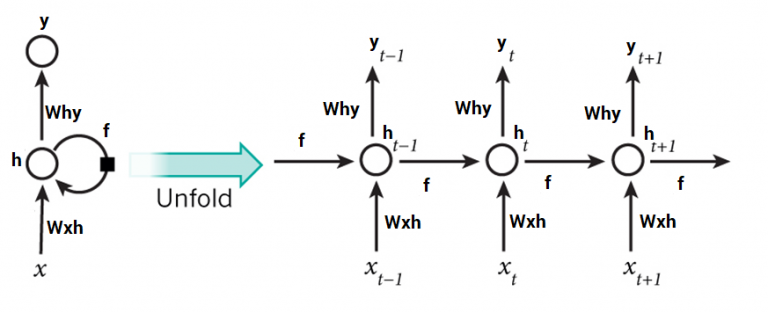
\includegraphics[width=0.8\linewidth,keepaspectratio]{rnn1}
\end{center}
  \begin{itemize}
  \item Every prediction at time t is dependent on the current input
  \item It also depends on all previous predictions and the information learned from them in form of hidden states.
   	  \end{itemize}

 \end{frame} 
 
   %%%%%%%%%%%%%%%%%%%%%%%%%%%%%%%%%%%%%%%%%%%%%%%%%%%%%%%%%%%%%%%%%%%%%%%%%%%%%%%%%%
\begin{frame}[fragile]
  \frametitle{Brief Review of Recurrent Neural Networks (RNN)}

  \begin{itemize}
  \item RNNs can solve our purpose of sequence handling to a great extent but not entirely. They are ok for short contexts.
  \item Single sentece coontext like \textbf{The color of the sky is \_\_\_}. Here we dont need to look back at previous sentences.
  
  	  \end{itemize}
  	   \begin{center}
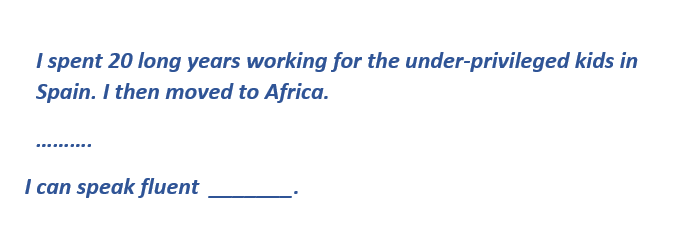
\includegraphics[width=0.8\linewidth,keepaspectratio]{rnn2}
\end{center}
 \end{frame} 
 
 
 
   %%%%%%%%%%%%%%%%%%%%%%%%%%%%%%%%%%%%%%%%%%%%%%%%%%%%%%%%%%%%%%%%%%%%%%%%%%%%%%%%%%
\begin{frame}[fragile]
  \frametitle{Brief Review of Recurrent Neural Networks (RNN)}
Vanishing Gradient
  \begin{itemize}
  \item In Back propogation weights are updated using gradient multiplied by learning rate.
  \item When dealing with activation functions like the sigmoid function, the small values of its derivatives gets multiplied multiple times as we move towards the starting layers. 
  \item As a result of this, the gradient almost vanishes as we move towards the starting layers, and it becomes difficult to train these layers.
  \item This issue can be resolved by applying a slightly tweaked version of RNNs - the Long Short-Term Memory Networks.
  	  \end{itemize}
 \end{frame} 
 
    %%%%%%%%%%%%%%%%%%%%%%%%%%%%%%%%%%%%%%%%%%%%%%%%%%%%%%%%%%%%%%%%%%%%%%%%%%%%%%%%%%
\begin{frame}[fragile]
  \frametitle{Brief Review of Recurrent Neural Networks (RNN)}

  \begin{itemize}
  \item In calendar, if in case we need to make some space for anything important we know which meeting could be canceled to accommodate a possible meeting.
  \item Turns out that an RNN doesn't do so. 
  \item In order to add a new information, it transforms the existing information completely by applying a function. 
    \item Because of this, the entire information is modified, on the whole, i. e. there is no consideration for 'important' information and 'not so important' information.
  	  \end{itemize}
 \end{frame} 
 
     %%%%%%%%%%%%%%%%%%%%%%%%%%%%%%%%%%%%%%%%%%%%%%%%%%%%%%%%%%%%%%%%%%%%%%%%%%%%%%%%%%
\begin{frame}[fragile]
  \frametitle{Brief Review of LSTM (Long Short-Term Memory) Networks}

  \begin{itemize}
  \item LSTMs on the other hand, make small modifications to the information by multiplications and additions. 
  \item With LSTMs, the information flows through a mechanism known as cell states. 
  \item This way, LSTMs can selectively remember or forget things. 
  \item The information at a particular cell state has three different dependencies.
  	  \end{itemize}
 \end{frame} 
 
      %%%%%%%%%%%%%%%%%%%%%%%%%%%%%%%%%%%%%%%%%%%%%%%%%%%%%%%%%%%%%%%%%%%%%%%%%%%%%%%%%%
\begin{frame}[fragile]
  \frametitle{Brief Review of LSTM (Long Short-Term Memory) Networks}

  \begin{itemize}
  \item Forget Gate: responsible for removing information from the cell state; example, previous subjects/objects are forgotten once new ones arrive.
    \item Input Gate: process of adding some new information to the cell state; example, adding more adjectives to same/current subject.
        \item Output Gate: selecting useful information from the current cell state and showing it out as an output;
  	  \end{itemize}
 \end{frame} 
 
      %%%%%%%%%%%%%%%%%%%%%%%%%%%%%%%%%%%%%%%%%%%%%%%%%%%%%%%%%%%%%%%%%%%%%%%%%%%%%%%%%%
\begin{frame}[fragile]
  \frametitle{Different Steps of Text Generation}
Text generation usually involves the following steps:
  \begin{itemize}
  \item Importing Dependencies
  \item Loading of Data
  \item Creating Character/Word mappings
  \item Data Preprocessing
  \item Modelling
  \item Generating text
  	  \end{itemize}
 \end{frame} 
 
 
%%%%%%%%%%%%%%%%%%%%%%%%%%%%%%%%%%%%%%%%%%%%%%%%%%%%%%%%%%%%%%%%%%%%%%%%%%%%%%%%%%
\begin{frame}[fragile]
  \frametitle{Shakespeare's Sonnets}
  \begin{itemize}
  \item Dataset: http://www.gutenberg.org/cache/epub/1041/pg1041.txt
\item Clean up, remove top and bottom irrelevant text and save it as ``sonnets.txt''
  	  \end{itemize}
\begin{lstlisting}
import numpy as np
import pandas as pd
from keras.models import Sequential
from keras.layers import Dense
from keras.layers import Dropout
from keras.layers import LSTM
from keras.utils import np_utils

text=(open("data/sonnets.txt").read())
text=text.lower()
print(text)
\end{lstlisting}
 \end{frame} 
 
%%%%%%%%%%%%%%%%%%%%%%%%%%%%%%%%%%%%%%%%%%%%%%%%%%%%%%%%%%%%%%%%%%%%%%%%%%%%%%%%%%
\begin{frame}[fragile]
  \frametitle{Creating character/word mappings}
  \begin{itemize}
  \item Machines understand only numbers
  \item So, each unique word/character is mapped to an id
  	  \end{itemize}
\begin{lstlisting}
characters = sorted(list(set(text)))
n_to_char = {n:char for n, char in enumerate(characters)}
char_to_n = {char:n for n, char in enumerate(characters)}
\end{lstlisting}
 \end{frame} 
  
%%%%%%%%%%%%%%%%%%%%%%%%%%%%%%%%%%%%%%%%%%%%%%%%%%%%%%%%%%%%%%%%%%%%%%%%%%%%%%%%%%
\begin{frame}[fragile]
  \frametitle{Creating character/word mappings}

  \begin{itemize}
  \item Using character level mappings and not word mappings. 
  \item word-based model shows much higher accuracy 
  \item But since this is a small dataset (with 17,670 words), and the number of unique words (4,605 in number) constitute around one-fourth of the data, it would not be a wise decision to train on such a mapping.
  \item This is because if we assume that all unique words occurred equally in number (which is not true), we would have a word occurring roughly four times in the entire training dataset, which is just not sufficient to build a text generator.
  	  \end{itemize}
 \end{frame} 
 
 %%%%%%%%%%%%%%%%%%%%%%%%%%%%%%%%%%%%%%%%%%%%%%%%%%%%%%%%%%%%%%%%%%%%%%%%%%%%%%%%%%
\begin{frame}[fragile]
  \frametitle{Data preprocessing}
  \begin{itemize}
  \item Most tricky part when it comes to building LSTM models. 
\item Transforming the data at hand into a relatable format is a difficult task.
  	  \end{itemize}
\begin{lstlisting}
X = []
Y = []
length = len(text)
seq_length = 100
for i in range(0, length-seq_length, 1):
    sequence = text[i:i + seq_length]
    label =text[i + seq_length]
    X.append([char_to_n[char] for char in sequence])
    Y.append(char_to_n[label])
\end{lstlisting}
 \end{frame} 
 
 %%%%%%%%%%%%%%%%%%%%%%%%%%%%%%%%%%%%%%%%%%%%%%%%%%%%%%%%%%%%%%%%%%%%%%%%%%%%%%%%%%
\begin{frame}[fragile]
  \frametitle{Creating character/word mappings}

  \begin{itemize}
  \item X is train array, and Y is  target array.
  \item X is of seq\_length and target is the next character.
  \item For a sequence length of 4 and the text ``hello india'', we would have our X and Y (not encoded as numbers for ease of understanding) as below:
    \begin{itemize}
  \item \lstinline| [h, e, l, l]	[o]|
  \item \lstinline| [e, l, l, o]	[ ]|
  \item \lstinline| [l, l, o,  ]	[i]|
  \item \lstinline| [l, o,  , i]	[n]|
  	  \end{itemize}
  	  \end{itemize}  	  
 \end{frame} 
 
  %%%%%%%%%%%%%%%%%%%%%%%%%%%%%%%%%%%%%%%%%%%%%%%%%%%%%%%%%%%%%%%%%%%%%%%%%%%%%%%%%%
\begin{frame}[fragile]
  \frametitle{Creating character/word mappings}

  \begin{itemize}
  \item LSTMs accept input in the form of \lstinline|(number_of_sequences, length_of_sequence, number_of_features) |which is not the current format of the arrays. 
  \item Also, we need to transform the array Y into a one-hot encoded format.
  	  \end{itemize}  	  
  	  
\begin{lstlisting}
X_modified = np.reshape(X, (len(X), seq_length, 1))
X_modified = X_modified / float(len(characters))
Y_modified = np_utils.to_categorical(Y)
\end{lstlisting}  	  
 \end{frame} 
 
   %%%%%%%%%%%%%%%%%%%%%%%%%%%%%%%%%%%%%%%%%%%%%%%%%%%%%%%%%%%%%%%%%%%%%%%%%%%%%%%%%%
\begin{frame}[fragile]
  \frametitle{Creating character/word mappings}

  \begin{itemize}
  \item Scale the values of our X\_modified so that our neural network can train faster and there is a lesser chance of getting stuck in a local minima. 
  \item Also, our Y\_modified is one-hot encoded to remove any ordinal relationship that may have been introduced in the process of mapping the characters. 
  	  \end{itemize}  	  
  	  
\begin{lstlisting}
X_modified = np.reshape(X, (len(X), seq_length, 1))
X_modified = X_modified / float(len(characters))
Y_modified = np_utils.to_categorical(Y)
\end{lstlisting}  	  

 \end{frame} 
 
    %%%%%%%%%%%%%%%%%%%%%%%%%%%%%%%%%%%%%%%%%%%%%%%%%%%%%%%%%%%%%%%%%%%%%%%%%%%%%%%%%%
\begin{frame}[fragile]
  \frametitle{Creating character/word mappings}
Final arrays will look like:
\begin{center}
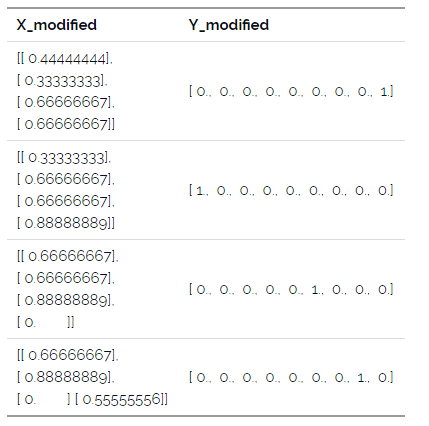
\includegraphics[width=0.5\linewidth,keepaspectratio]{rnn3}
\end{center}
 \end{frame} 
 
%%%%%%%%%%%%%%%%%%%%%%%%%%%%%%%%%%%%%%%%%%%%%%%%%%%%%%%%%%%%%%%%%%%%%%%%%%%%%%%%%%
\begin{frame}[fragile]
  \frametitle{Modelling}

  \begin{itemize}
  \item Building a sequential model with two LSTM layers having 400 units each. 
  \item The first layer needs to be fed in with the input shape. 
  \item In order for the next LSTM layer to be able to process the same sequences, we enter the return\_sequences parameter as True.
\item Also, dropout layers with a 20\% dropout have been added to check for over-fitting. 
\item The last layer outputs a one hot encoded vector which gives the character output.
  	  \end{itemize}  	  
  	  
\end{frame} 
 
%%%%%%%%%%%%%%%%%%%%%%%%%%%%%%%%%%%%%%%%%%%%%%%%%%%%%%%%%%%%%%%%%%%%%%%%%%%%%%%%%%
\begin{frame}[fragile]
  \frametitle{Modelling}
  	  
\begin{lstlisting}
model = Sequential()
model.add(LSTM(400, input_shape=(X_modified.shape[1], X_modified.shape[2]), return_sequences=True))
model.add(Dropout(0.2))
model.add(LSTM(400))
model.add(Dropout(0.2))
model.add(Dense(Y_modified.shape[1], activation='softmax'))
model.compile(loss='categorical_crossentropy', optimizer='adam')
\end{lstlisting}  	  

 \end{frame} 
  
 %%%%%%%%%%%%%%%%%%%%%%%%%%%%%%%%%%%%%%%%%%%%%%%%%%%%%%%%%%%%%%%%%%%%%%%%%%%%%%%%%%
\begin{frame}[fragile]
  \frametitle{Generating Text}
\begin{lstlisting}
string_mapped = X[99]
# generating characters
for i in range(seq_length):
    x = np.reshape(string_mapped,(1,len(string_mapped), 1))
    x = x / float(len(characters))
    pred_index = np.argmax(model.predict(x, verbose=0))
    seq = [n_to_char[value] for value in string_mapped]
    string_mapped.append(pred_index)
    string_mapped = string_mapped[1:len(string_mapped)]
\end{lstlisting}  	  

 \end{frame}  
 
 % %%%%%%%%%%%%%%%%%%%%%%%%%%%%%%%%%%%%%%%%%%%%%%%%%%%%%%%%%%%%%%%%%%%%%%%%%%%%%%%%%%
% \begin{frame}[fragile]
  % \frametitle{Generating Text}
    % \begin{itemize}
  % \item We start off with a random row from the X array, that is an array of 100 characters. 
  % \item After this, we target predicting another 100 characters following X. 
  % \item The input is reshaped and scaled as previously and the next character with maximum probability is predicted.
  % \item seq is used to store the decoded format of the string that has been predicted till now. 
  % \item Next, the new string is updated, such that the first character is removed and the new predicted character is included.
% \end{itemize}  	  
% \end{frame}    	
 
% % %%%%%%%%%%%%%%%%%%%%%%%%%%%%%%%%%%%%%%%%%%%%%%%%%%%%%%%%%%%%%%%%%%%%%%%%%%%%%%%%%%
% % \begin{frame}[fragile]
  % % \frametitle{Experimenting with different models}
  % % The baseline model, when trained for 1 epoch with a batch size of 100, gave the following output:
% % \begin{lstlisting}
% % 's the riper should by time decease,
% % his tender heir might bear his memory:
% % but thou, contracted toet she the the the the the the the the
% % thi the the the the the the the the the the the the the the the the the
% % thi the the the the the the the the the the the the the the the the the
% % thi the the the the the the the the the the the the the the the the the
% % thi the the the the the the the the the the the the the the the the the
% % thi the the the the the the the the th'
% % \end{lstlisting}  	  
% % \end{frame}     
 
  % % %%%%%%%%%%%%%%%%%%%%%%%%%%%%%%%%%%%%%%%%%%%%%%%%%%%%%%%%%%%%%%%%%%%%%%%%%%%%%%%%%%
% % \begin{frame}[fragile]
  % % \frametitle{Experimenting with different models}
 	  
% % This output doesn't make much sense. It is nothing but a repetition of the same prediction, as if it's stuck in a loop. This is because language prediction models are way too complex when compared to the miniature model that we have trained.
 % % \end{frame}     
  
 % % %%%%%%%%%%%%%%%%%%%%%%%%%%%%%%%%%%%%%%%%%%%%%%%%%%%%%%%%%%%%%%%%%%%%%%%%%%%%%%%%%%
% % \begin{frame}[fragile]
  % % \frametitle{A more trained model}
% % This time we trained our model for 100 epochs and a batch size of 50. We at least obtained a non-repetitive sequence of characters, which contains a decent number of legitimate words. Also, the model learnt to produce a sonnet-like word structure.
% % \begin{lstlisting}
% % 'The riper should by time decease,
% % his tender heir might bear his memory:
% % but thou, contracted to thine own besire,
% % that in the breath ther doomownd wron to ray,
% % dorh part nit backn oy steresc douh dxcel;
% % for that i have beauty lekeng norirness,
% % for all the foowing of a former sight,
% % which in the remame douh a foure to his,
% % that in the very bumees of toue mart detenese;
% % how ap i am nnw love, he past doth fiamee.
% % to diserace but in the orsths of are orider,
% % waie agliemt would have me '
% % \end{lstlisting}  	  
% % However, this model is still not good enough to produce quality content. Build a deeper architecture!
 % % \end{frame}     
 
 
  
 % % %%%%%%%%%%%%%%%%%%%%%%%%%%%%%%%%%%%%%%%%%%%%%%%%%%%%%%%%%%%%%%%%%%%%%%%%%%%%%%%%%%
% % \begin{frame}[fragile]
  % % \frametitle{A deeper model}
% % Let's add another LSTM layer with 400 units followed by a dropout layer of 0.2 fraction and see what we get.
% % \begin{lstlisting}
% % "The riper should by time decease,
% % his tender heir might bear his memory:
% % but thou, contracted to the world's false sporoe,
% % with eyes so dond touls be thy domfornds,
% % which for memorion of the seasons new;
% % mike own self-love to shou art constant
% % how can i then be oy love doth give,
% % the rose looks fair, but fairer bomments age.
% % now with the seas that i have seen dychl
% % that mot to teed of you, if h ho bontent,
% % and all the ress of the heartai thee;
% % the world will was iis bound and farty "
% % \end{lstlisting}  	  

 % % \end{frame}   
 
   
 % % %%%%%%%%%%%%%%%%%%%%%%%%%%%%%%%%%%%%%%%%%%%%%%%%%%%%%%%%%%%%%%%%%%%%%%%%%%%%%%%%%%
% % \begin{frame}[fragile]
  % % \frametitle{A deeper model}
 
    % % \begin{itemize}
  % % \item The grammar has enhanced itself, keeping the sonnet structure and punctuation intact. 
  % % \item However, this still requires a lot of improvement. 
  % % \item Let's try and explore a wider network, one with more number of units.
    % % \end{itemize}          
 % % \end{frame}   
 
 % % %%%%%%%%%%%%%%%%%%%%%%%%%%%%%%%%%%%%%%%%%%%%%%%%%%%%%%%%%%%%%%%%%%%%%%%%%%%%%%%%%%
% % \begin{frame}[fragile]
  % % \frametitle{A wider model}
% % I increased the number of units to 700 on each of the two LSTM layers. This tweak produced the following poetry:
% % \begin{lstlisting}
% % "The riper should by time decease,
% % his tender heir might bear his memory:
% % but thou, contracted to thine own bright eyes,
% % feed'st thy sigh aare so beuider poise,
% % oor maty dis surre that gairs mot me love thee;
% % when i braye the would and lays in the eesire.
% % than thmu disgrmed stand with my bootr still nsentente;
% % tell ia to thou art thou wilt woon'thy sook,
% % and touain then tor, give thy soue semping.
% % whose whod the better of your befaiss nu sante,
% % though i, suoll oas, and i lose bouh twa"
% % \end{lstlisting}  	  

 % % \end{frame}       
 
  % % %%%%%%%%%%%%%%%%%%%%%%%%%%%%%%%%%%%%%%%%%%%%%%%%%%%%%%%%%%%%%%%%%%%%%%%%%%%%%%%%%%
% % \begin{frame}[fragile]
  % % \frametitle{A wider model}
    % % \begin{itemize}
  % % \item This is a little disappointing at first, because the words have lost their meaning. 
  % % \item But, what's interesting to note here is that there is some rhyme that is building up. 
    % % \item The model is trying to understand poetry after all! 
      % % \item But, we cannot compromise with meaningful words, right? 
        % % \item Let's put it all together in a one gigantic model.
    % % \end{itemize}        
 % % \end{frame}    
 
  
 % % %%%%%%%%%%%%%%%%%%%%%%%%%%%%%%%%%%%%%%%%%%%%%%%%%%%%%%%%%%%%%%%%%%%%%%%%%%%%%%%%%%
% % \begin{frame}[fragile]
  % % \frametitle{A gigantic model}
% % I increased the number of layers to three, each having 700 units and trained it for 100 epochs. The result produced is a magnificent piece of poetry. Take a look:
% % \begin{lstlisting}
% % "The riper should by time decease,
% % his tender heir might bear his memory:
% % but thou, contracted to thine own bright eyes,
% % feed'st thy light's flame with self-substantial fuel,
% % my beept is she breat oe bath dasehr ill:
% % tirse do i pine and turfeit day by day,
% % or gluttoning on all, or all away.
% % Lxxvi
% % why is my verse so barren of new pride,
% % so far from variation or quick change?
% % why with the time do i not glance aside
% % to new-found methods, and to compounds strange?
% % why write i stil"
% % \end{lstlisting}  	  

 % % \end{frame}   
 
   
 % % %%%%%%%%%%%%%%%%%%%%%%%%%%%%%%%%%%%%%%%%%%%%%%%%%%%%%%%%%%%%%%%%%%%%%%%%%%%%%%%%%%
% % \begin{frame}[fragile]
  % % \frametitle{A gigantic model}
  
  % % \begin{itemize}
  % % \item This not only has sensible words, but has also learnt to rhyme. 
    % % \item We could have had a more sensible piece of art had the data that was fed into the network been cleaned properly! 
      % % \item But as a starting piece, this model has more than done what it was asked. 
        % % \item It is way more poetic than most humans could ever get!
    % % \end{itemize}                
 % % \end{frame}   
 
  % % %%%%%%%%%%%%%%%%%%%%%%%%%%%%%%%%%%%%%%%%%%%%%%%%%%%%%%%%%%%%%%%%%%%%%%%%%%%%%%%%%%
% % \begin{frame}[fragile]
  % % \frametitle{End Notes}
  % % \begin{itemize}
  % % \item What makes a text generator more efficient is its capability to generate relevant stories.
  % % \item Andrej Karpathy's character level RNN model is one such masterpiece, a sufficiently trained model on this framework gives some eye-popping results.
  	  % % \end{itemize}
 % % \end{frame}   
